%\documentclass[12pt,a4paper]{scrbook}
%\usepackage[utf8]{inputenc}
%\usepackage{amsmath}
%\usepackage{amsfonts}
%\usepackage{amssymb}
%\usepackage{graphicx}
%\usepackage{csquotes}

%\begin{document}
	
\chapter{Fachschaftika? Kann man das essen?}

\section{Die Fachschaft}
Wir sind die Gruppe Aktiver Fachschaftika, oder kurz GAF. Ein Fachschaftikon ist ein Mitglied einer Fachschaft, das sind alle Studika eines Studiengangs, also auch du, ob du willst oder nicht. Spricht man über \emph{die Fachschaft}, meint man damit meist die aktiven Fachschaftika, die versuchen, die Uni für alle Studika lebenswerter zu machen. Die GAF ist der Zusammenschluss aus aktiven Fachschaftika der Fachbereiche Mathematik, Physik und Informatik, sowie der verwandten Fächer (Medieninformatik, Wirtschaftsmathematik\ldots).

\section{Aufgaben der Fachschaft}

Was die Fachschaft tut, lässt sich grob in zwei Bereiche teilen: einerseits vertritt sie die Studika zur Seite der Fakultät hin, andererseits kümmert sie sich um die Studika selbst.

Durch Repräsentation in verschiedenen Gremien verleiht sie der Meinung und den Interessen der Studika Gewicht und versucht so, Entscheidungen über die Köpfe der Studika hinweg zu unterbinden. Einige der wichtigsten Gremien haben wir hier aufgelistet.
Der \emph{Fakulträtsrat} entscheidet alles Wichtige innerhalb der Fakultät und ist Ort des Informationsaustausches.
Die \emph{Studienzuschusskommission} beschließt, wofür Geld ausgegeben wird.
Die \emph{Berufungskommissionen} bestimmen, wer als neues Professorikon an unsere Uni kommt und hier auch lehrt.
Der \emph{Konvent der Fachschaften} besteht aus Vertretern aller Fachschaften und beschäftigt sich mit fächerübergreifenden, studentischen Themen

Außerdem versuchen wir euch Studika das Unileben zu erleichtern. Wir sammeln Altklausuren und Prüfungsprotokolle\footnote{Beachte hier den Generationenvertrag: die Sammlung existiert nur, weil ältere Studika ihre Prüfungen zu uns gebracht haben, also tu dies auch für deine Nachfolger!} und stehen als Ansprechpartner für Probleme, bei denen du nicht weißt, an wen du dich wenden sollst, zur Verfügung. Gerne unterstützen wir dich auch bei der Umsetzung deiner Ideen durch tatkräftige Mitarbeit und Know-How. Schließlich sorgen wir noch für Bespaßung, zum Beispiel durch das alljährliche Fakultätsfest.

Wenn du dir selbst einen Eindruck von unserer Arbeit verschaffen willst, melde dich zum EWO (Ersti-Wochenende) an, komme bei uns im Büro vorbei oder auf eine Sitzung. Die Termine dafür findest du unter \ref{gaf}.

Wichtig zu wissen ist, dass wir das alles ehrenamtlich machen und das Geld, das uns zur Verfügung steht, nur zugunsten der Studika einsetzen. Der einzige Lohn unserer Arbeit ist mehr Lebenserfahrung und in manchen Fällen ein verlängertes Studium.

\begin{urlList}
	\urlItem{https://gaf.fs.lmu.de}[gaf]
\end{urlList}

\section{Kontakt}\label{gafKontakt}
%XXX To do: seperate Box/ optisch aufwerten
\begin{tabular}{ l l l l }
Telefon&089 / 2180\emd{}4382\\
Telefax&089 / 2180\emd{}4391\\
&\\
&\mail{gaf@fs.lmu.de}\\
&\mail{gumbel@fs.lmu.de}\\
&\\
&\url{\https gaf.fs.lmu.de}\\
&\url{\https facebook.com/gaflmu}\\
&\\
IRC & \#gaf auf freenode
\end{tabular}

\section{Andere Fachschaften}
\begin{urlList}
	\urlItem{https://mi.fs.lmu.de}
	\urlItem{http://www.bioinformatik-muenchen.com/bioinfocom/fachschaft/}
	\urlItem{http://www.meteo.physik.lmu.de/~studmet}
        \urlItem{http://www.statistik.lmu.de/~fachsch/}
\end{urlList}

\skiptobottom
\centerline{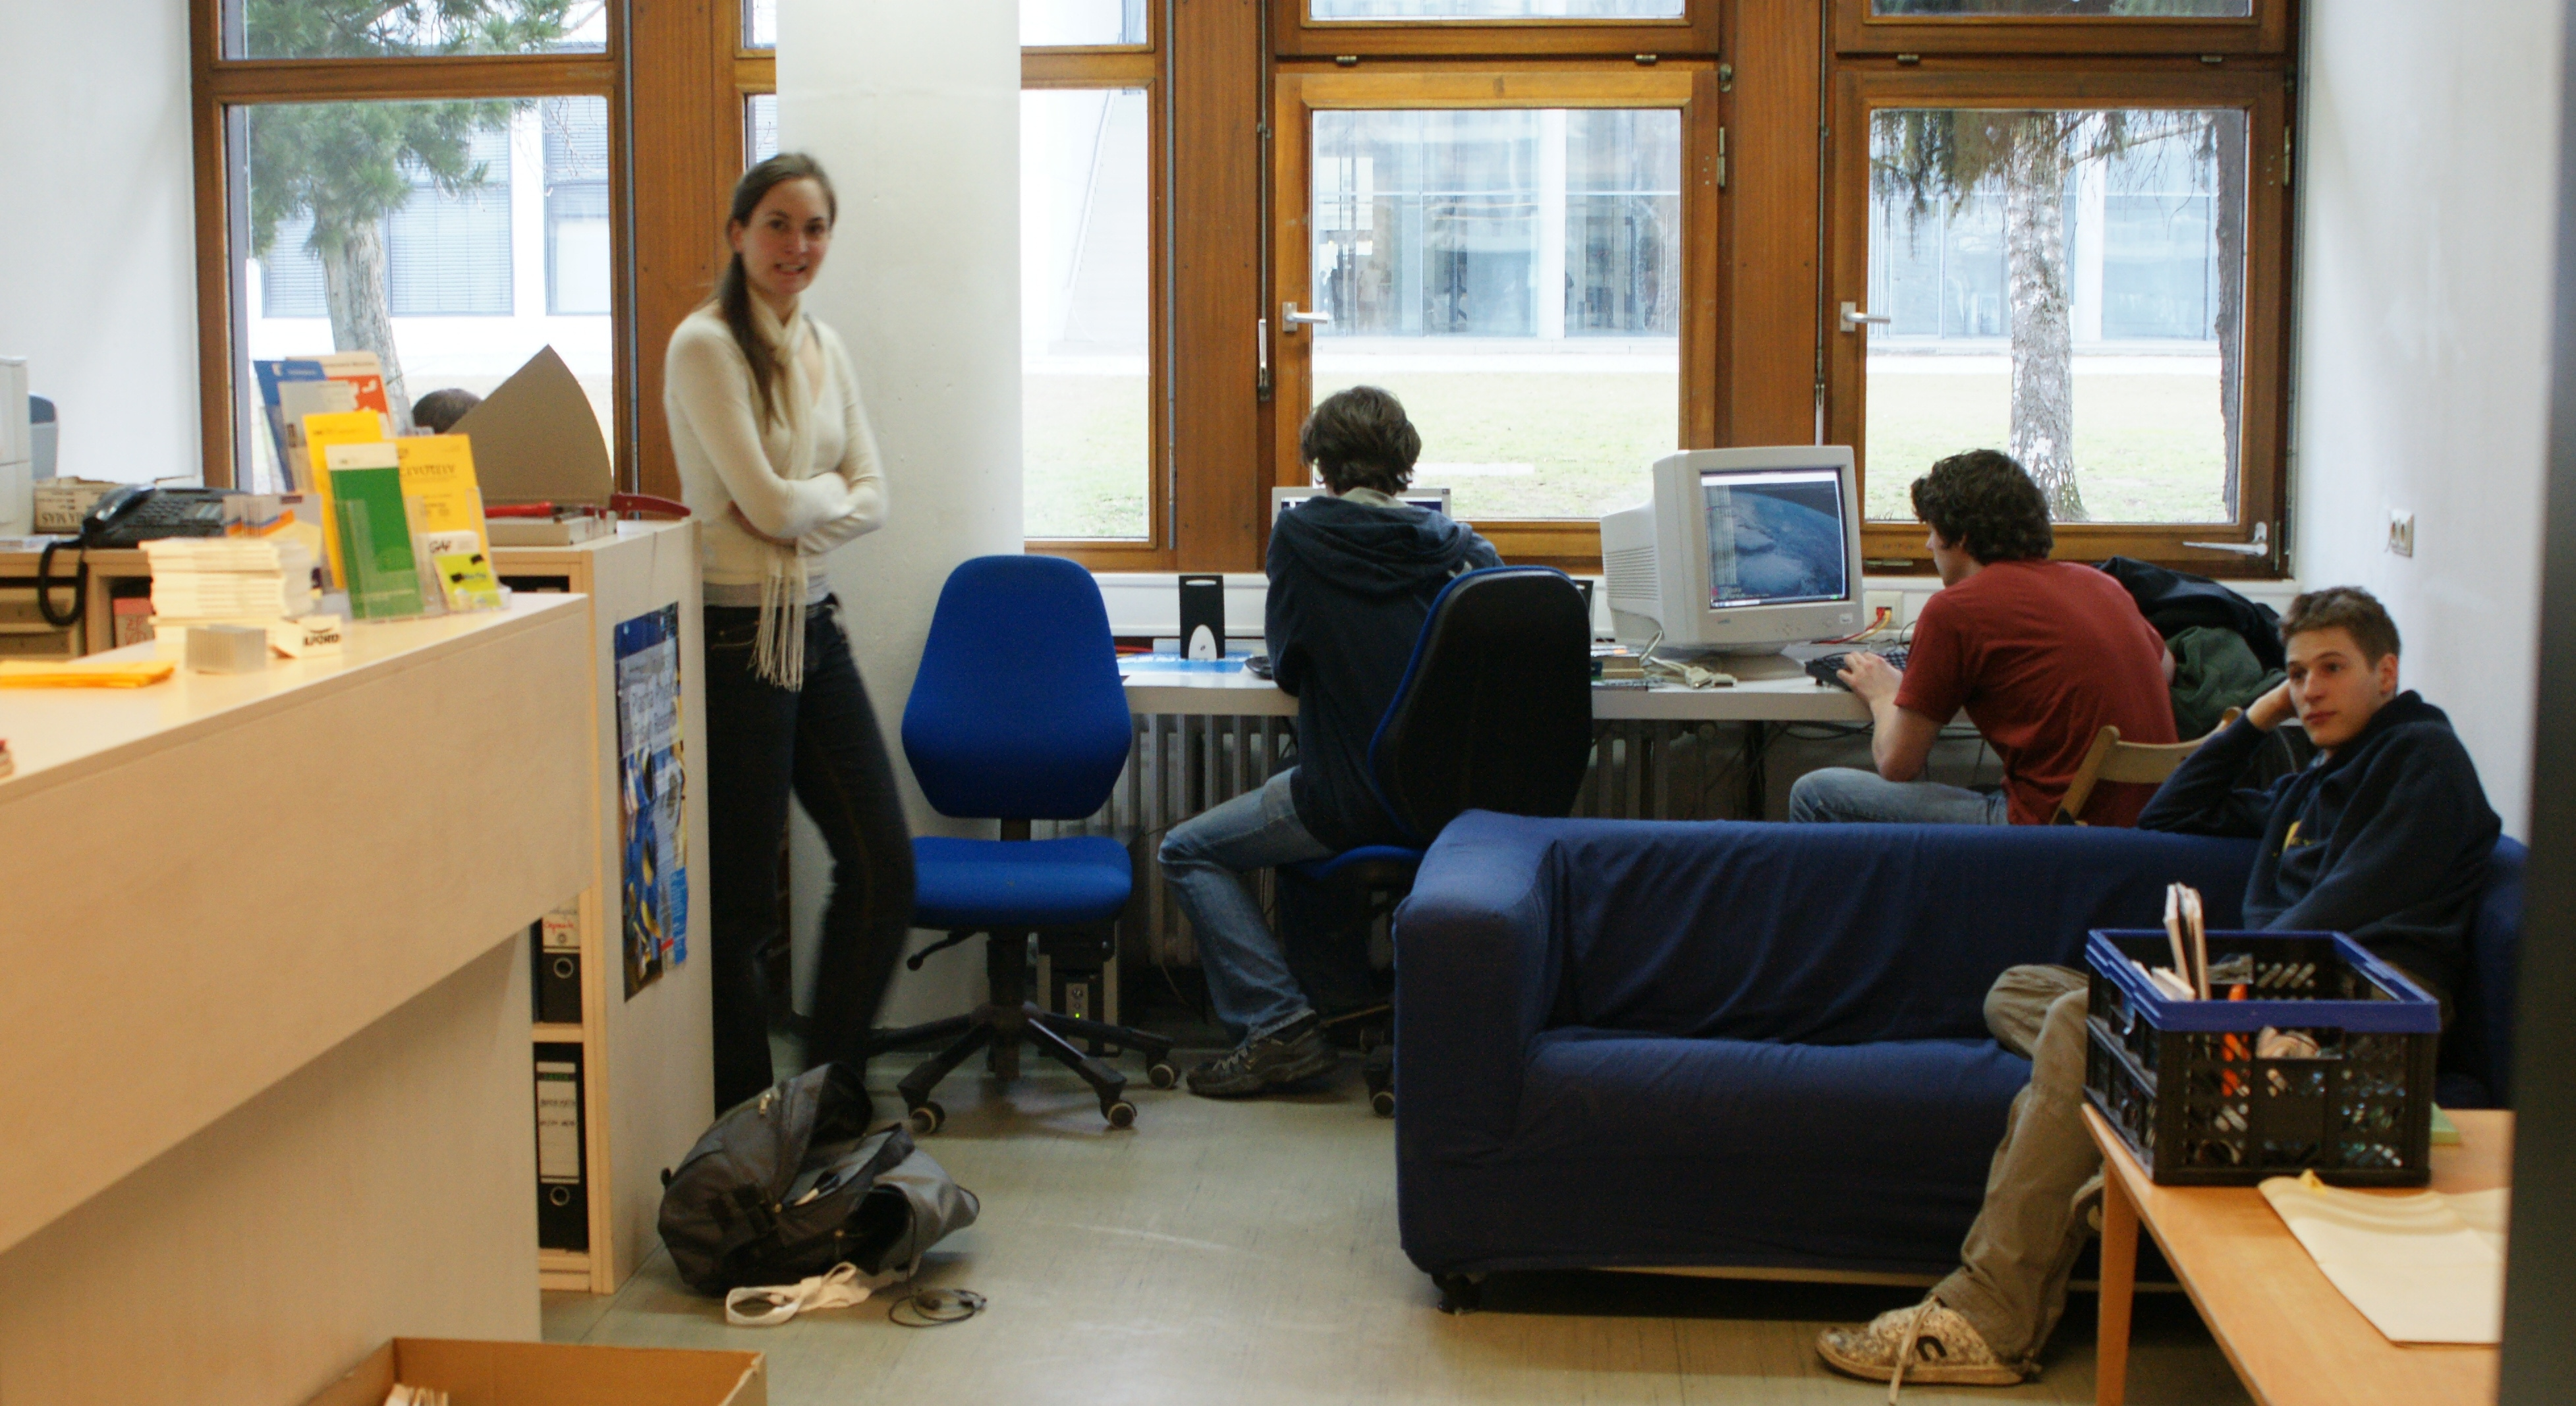
\includegraphics[width=0.8\textwidth]{aktive-fachschaft_print}}

%\end{document}
